\documentclass[11pt,a4paper]{article}

\usepackage[margin=2.2cm]{geometry}
\usepackage[T1]{fontenc}
\usepackage{lmodern}
\usepackage{amssymb}
\usepackage{xcolor}
\usepackage{tikz}
\usetikzlibrary{arrows.meta,positioning}
\usepackage{booktabs}
\usepackage{tabularx}
\usepackage{enumitem}
\usepackage{listings}
\usepackage[most]{tcolorbox}
\usepackage{fancyhdr}
\usepackage[colorlinks=true,linkcolor=blue!50!black,urlcolor=blue!50!black]{hyperref}

\definecolor{local}{HTML}{2E7D32}
\definecolor{cloud}{HTML}{1565C0}
\definecolor{warn}{HTML}{C62828}
\definecolor{idea}{HTML}{6A1B9A}
\definecolor{soft}{HTML}{F5F5F5}

\newtcolorbox{concept}[1]{colback=idea!4,colframe=idea!70,fonttitle=\bfseries,title={Concept: #1},breakable}
\newtcolorbox{analogy}{colback=local!5,colframe=local!70,fonttitle=\bfseries,title={Analogy},breakable}
\newtcolorbox{why}{colback=cloud!4,colframe=cloud!70,fonttitle=\bfseries,title={Why it is done this way},breakable}
\newtcolorbox{caution}{colback=warn!4,colframe=warn!70,fonttitle=\bfseries,title={Watch out},breakable}
\newtcolorbox{exercise}{colback=soft,colframe=black!50,fonttitle=\bfseries,title={Check yourself},breakable}

\lstset{basicstyle=\ttfamily\small,backgroundcolor=\color{soft},frame=single,
        rulecolor=\color{black!25},columns=fullflexible,keepspaces=true,
        showstringspaces=false,breaklines=true}

\pagestyle{fancy}
\fancyhf{}
\lhead{\small Listen -- Learning Doc 06}
\rhead{\small The Sync Protocol}
\cfoot{\thepage}

\title{\textbf{Listen}\\[4pt]\large Learning Doc 06: The Sync Protocol\\
       \normalsize Keeping a laptop and a server in agreement, cheaply and offline-first}
\author{Detailed design, Section 5}
\date{13 October 2026}

\begin{document}
\maketitle

\begin{abstract}
\noindent Your laptop and the cloud each hold a copy of some data. This document designs how
those copies stay in agreement: what is sent, when, in which direction, what happens when
you are offline, when the same message arrives twice, when you delete something, and when you
edit the same command on both sides. The whole exchange is one small request every five
minutes.
\end{abstract}

\tableofcontents
\newpage

% =====================================================================
\section{Decisions this section is built on}
\begin{center}
\renewcommand{\arraystretch}{1.2}
\begin{tabularx}{\textwidth}{l X}
\toprule
\textbf{Topic} & \textbf{Decision} \\
\midrule
Command files     & The YAML files on the laptop are the master, kept in the repository's \texttt{commands/} folder (versioned in git). They can be edited in PyCharm \emph{or} in the web app; web edits are written into the YAML. \\
Reconnecting      & Sync immediately when Windows reports the network is back. \\
Conflicts         & If both sides changed the same command, the laptop version wins. \\
Frequency         & Every 5 minutes. Lightweight first. The dashboard refreshes every 5 minutes too. \\
Deleting history  & From the review list and the web app (no voice). A deletion on one side reaches the other. \\
Privacy (Doc 05)  & Only syncable tables are ever read by the sync code. \\
\bottomrule
\end{tabularx}
\end{center}

% =====================================================================
\section{Who talks to whom}

\begin{concept}{Polling}
The server cannot contact your laptop: your laptop sits behind home Wi-Fi with no public
address, and may be off. So the laptop \textbf{polls}: every 5 minutes \emph{it} contacts the
server, sends what is new, and asks ``anything new for me?''. The server only ever answers.
\end{concept}

\begin{analogy}
A post office box. The post office cannot deliver to a house it cannot find, so it keeps your
mail in a box. Every so often you visit, drop off your outgoing letters and collect what is
waiting. If you are away for a week, the mail simply waits.
\end{analogy}

\begin{center}
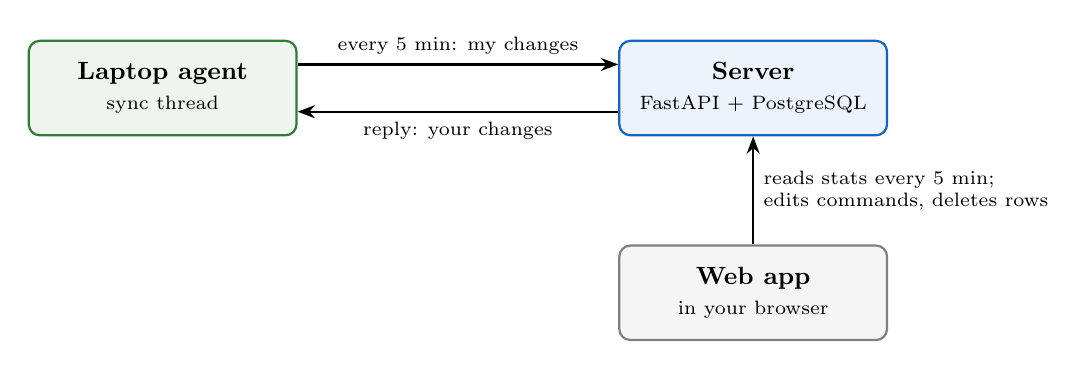
\begin{tikzpicture}[font=\small,
  box/.style={draw,rounded corners=4pt,minimum width=3.4cm,minimum height=1.2cm,align=center,thick},
  arr/.style={-{Stealth[length=2.2mm]},thick}]
\node[box,draw=local,fill=local!8] (l) at (0,0) {\textbf{Laptop agent}\\\scriptsize sync thread};
\node[box,draw=cloud,fill=cloud!8] (s) at (7.5,0) {\textbf{Server}\\\scriptsize FastAPI + PostgreSQL};
\node[box,draw=black!50,fill=soft] (w) at (7.5,-2.6) {\textbf{Web app}\\\scriptsize in your browser};
\draw[arr] ([yshift=3mm]l.east) -- node[above,font=\scriptsize]{every 5 min: my changes} ([yshift=3mm]s.west);
\draw[arr] ([yshift=-3mm]s.west) -- node[below,font=\scriptsize]{reply: your changes} ([yshift=-3mm]l.west -| l.east);
\draw[arr] (w) -- node[right,font=\scriptsize,align=left]{reads stats every 5 min;\\edits commands, deletes rows} (s);
\end{tikzpicture}
\end{center}

% =====================================================================
\section{One round trip every 5 minutes}

Each sync is a \textbf{single HTTPS request} carrying everything the laptop has to say, and a
single reply carrying everything the server has to say. One request instead of five separate
ones keeps the network use and battery cost close to zero.

\begin{lstlisting}
POST /sync                                   (laptop -> server)
{
  "cursor": 1841,                    # "I have seen server changes up to #1841"
  "rows":      [ ...new or changed commands / usage_daily rows... ],
  "deletions": [ "uuid-1", "uuid-2" ],          # rows you deleted locally
  "commands_snapshot": { "hash": "a91f...", "files": {...} },  # only if changed
  "edit_results": [ {"edit": 17, "status": "applied"} ]
}

reply                                        (server -> laptop)
{
  "accepted":  [ "uuid-...", ... ],          # rows the server stored
  "deletions": [ "uuid-9" ],                 # rows you deleted in the web app
  "pending_edits": [ {...an edit made in the web app...} ],
  "cursor": 1856
}
\end{lstlisting}

\noindent When nothing has changed, the request is a few hundred bytes. When the laptop is
offline, nothing is lost: unsent rows simply stay unsent until the next successful sync.

% =====================================================================
\section{Uploading history: safe even when messages repeat}

\paragraph{What needs sending.} A row in a syncable table needs uploading if it was never
sent (\texttt{synced\_at} is empty) or it changed since it was sent
(\texttt{updated\_at} \textgreater{} \texttt{synced\_at}). The second case matters: when you mark
a command wrong, or today's usage total grows, the row changes \emph{after} it was uploaded.

\paragraph{Batches.} At most 500 rows per request; if there are more (after a week offline),
the next sync continues immediately until the backlog is gone. Why a limit at all? One huge
request after a long offline stretch would (1) lose \emph{all} progress if the connection drops
near the end, (2) risk hitting network and server time limits on slow Wi-Fi, and (3) need the
whole backlog in memory on both sides. With batches, every confirmed batch is permanently done.
Why 500: a row is about 0.5--1\,KB, so a batch is roughly 250--500\,KB, under a second on
ordinary internet. Fifty would mean dozens of round trips for a week's backlog; five thousand
brings back the problems above. It is a tunable starting value, and in normal use (0--20 rows
per sync) it never comes into play.

\begin{concept}{Outbox pattern (store and forward)}
There is no separate queue of ``messages to send''. The unsent data \emph{is} the rows
themselves, sitting in SQLite with \texttt{synced\_at} empty or older than \texttt{updated\_at};
``what to send'' is just a query. Nothing expires: rows wait for days or months if needed, and are
marked sent only after the server confirms them. The 30-day purge only touches the private
tables, which are never in the outbox at all.
\end{concept}

\begin{concept}{Idempotency}
An operation is \textbf{idempotent} if doing it twice has the same effect as doing it once.
Networks fail in an awkward way: the server may store your rows and then the reply is lost, so
the laptop thinks it failed and sends them again. Because every row carries its \texttt{uuid},
the server performs an \textbf{upsert} (``insert, or update if that uuid already exists''), so
receiving the same row twice changes nothing. That lets the laptop simply retry anything that
was not confirmed.
\end{concept}

\noindent After the reply arrives, the laptop sets \texttt{synced\_at} only on the uuids the
server listed as \texttt{accepted}.

\begin{concept}{Retry with back-off}
If a sync fails (no internet, server down), the next attempt waits longer: 5, 10, 20, then at
most 30 minutes. This is \textbf{exponential back-off}: it stops a laptop with no Wi-Fi from
wasting effort retrying every few seconds. One success resets it to 5 minutes.
\end{concept}

\paragraph{Back online: sync immediately (decided).} Waiting up to 30 minutes after the
internet returns is unnecessary. Windows announces network changes; the sync thread subscribes
to that notification and, when a connection appears, syncs at once instead of waiting for the
back-off timer. Subscribing costs nothing while waiting: Windows wakes the thread only when the
network actually changes.

% =====================================================================
\section{Deleting: tombstones}

If you delete a row locally and the laptop just forgets it, the next sync has nothing to tell
the server, and the server keeps the row forever. Deletions must be \emph{remembered} until
they have been delivered.

\begin{concept}{Tombstone}
A \textbf{tombstone} is a marker that says ``this row was deleted''. Instead of removing the row
immediately, Listen sets its \texttt{deleted\_at}. It disappears from every list at once,
but it still exists long enough for the sync to report its uuid. Once the other side confirms,
the row is removed for real.
\end{concept}

\paragraph{How long does each tombstone live?} There are two, and neither runs on a timer:
\begin{center}
\renewcommand{\arraystretch}{1.2}
\begin{tabularx}{\textwidth}{l X X}
\toprule
\textbf{Where} & \textbf{What is kept} & \textbf{Removed when} \\
\midrule
Laptop (\texttt{deleted\_at}) & The whole row, hidden everywhere &
As soon as the server confirms the deletion: the next successful sync (usually within 5 minutes,
or right after reconnecting). Event-based, not time-based. \\
Server (\texttt{tombstones}) & Only the uuid and the deletion time ($\approx$40 bytes), \emph{no content} &
Kept indefinitely, so even a laptop offline for months cannot resurrect the row. Ten thousand
deletions $\approx$ 400\,KB. \\
\bottomrule
\end{tabularx}
\end{center}
\noindent The \emph{content} of a deleted command (what you said, its timings) leaves the server
the moment the deletion arrives. The server's tombstone remembers only that \emph{something with
this id} was deleted, never what it was.

\begin{itemize}[nosep]
  \item \textbf{Deleted in the review list:} tombstone locally $\to$ next sync sends the uuid
        $\to$ server deletes its copy $\to$ laptop removes the row.
  \item \textbf{Deleted in the web app:} server removes it and records the deletion in its
        change log $\to$ next sync returns the uuid $\to$ laptop removes its copy.
\end{itemize}

\paragraph{The resurrection problem, and the server's tombstones.} A tombstone is crossing an
entry out of a shared notebook instead of tearing the page out: anyone reading later still learns
it was deleted. Consider this sequence:
\begin{enumerate}[nosep]
  \item Monday: a command syncs to the server.
  \item Tuesday: you delete it in the web app; the server removes it.
  \item Tuesday evening, offline: you mark that same command ``wrong'' in the review list, so its
        \texttt{updated\_at} changes and the laptop wants to re-upload it.
  \item Wednesday: the upload arrives; an upsert finds no such row and \emph{inserts it again}.
        Your deleted command is back.
\end{enumerate}
\noindent To prevent this, the server also keeps a tombstone (the uuid and the deletion time, about
40 bytes, kept indefinitely). Any upload of a tombstoned uuid is refused, and the laptop removes
its copy when it receives the deletion.

\begin{concept}{Cursor (change log)}
The server numbers every change it makes (``change \#1856: row uuid-9 deleted''). The laptop
remembers the last number it has seen, the \textbf{cursor}. Each sync asks for ``everything
after \#1841''. Nothing is missed, nothing is sent twice, and the server does not have to
remember which laptop has seen what: the laptop keeps its own place, like a bookmark.
\end{concept}

\noindent \textbf{Where it lives:} the numbered change log is on the server; the cursor is on the
laptop, in the \texttt{meta} table. Like a book: the publisher prints the page numbers, each
reader keeps a bookmark. A second device would simply have its own bookmark, and if the laptop's
database were lost, the cursor restarts at 0 and the laptop re-reads every change; nothing
breaks.

% =====================================================================
\section{Commands: two editors, one master}

Command files are different from history. History only ever flows \emph{up}. Commands can be
edited on \emph{both} sides, and only one copy can be the truth.

\subsection{Laptop $\to$ server: snapshots}
Whenever the command files change (you saved in PyCharm, or a web edit was applied), the next
sync includes a \textbf{snapshot}: the files' contents and a \textbf{hash}.

\begin{concept}{Hash}
A \textbf{hash} is a short fingerprint computed from content: change one character and the
fingerprint changes completely. Comparing two hashes tells you whether two files are identical
without comparing them line by line. The laptop only sends a snapshot when the hash differs from
the last one sent.
\end{concept}

\noindent The server stores the latest snapshot. The web app shows your commands from it.
It also includes the list of primitives your agent has (Doc~03 \S8), so the web app and the AI
command builder only offer actions that exist on your laptop.

\subsection{Server $\to$ laptop: edits wait to be applied}
A change made in the web app is \emph{not} applied on the server. It becomes a \textbf{pending
edit}: ``change command \texttt{play}: default target \texttt{spotify}'', recorded together with
the snapshot hash it was based on. On the next sync the laptop receives it and decides:

\begin{lstlisting}
for each pending edit:
    if the command it changes is identical to what the web app saw:
        write the change into the YAML file      # preserving your comments
        validate it (Doc 03); if invalid -> undo the write, status = "invalid"
        else status = "applied"                  # hot reload picks it up
    else:
        status = "overridden"                    # you changed it locally: laptop wins
report every status in the next sync
\end{lstlisting}

\noindent The web app shows each edit's status: \emph{waiting for laptop}, \emph{applied},
\emph{invalid}, or \emph{overridden by a change on your laptop}. ``Waiting for laptop'' does
\emph{not} ask you to confirm anything: it only means the edit is stored on the server and the
laptop has not collected it yet (it is offline, or the next sync has not happened). The laptop
applies it automatically; online, that takes at most about 5 minutes.

\paragraph{Edge case: the file is open in PyCharm.} Listen sees only what is saved on disk. If
you have \emph{unsaved} changes to the same file when a web edit is written, PyCharm notices the
file changed on disk and asks which version to keep. Nothing is lost silently.

\begin{concept}{Optimistic concurrency}
Rather than locking a command while someone edits it, each edit carries the version it was
based on, and is accepted only if that version is still current. It is ``optimistic'' because
it assumes conflicts are rare and only checks at the end. Git does the same when it refuses a
push because the remote has moved on.
\end{concept}

\begin{why}
This gives you exactly what you asked for. \textbf{Offline}, PyCharm editing always works,
because the files are on your laptop. \textbf{Web} editing works any time; the change lands
within 5 minutes of the laptop being online. And there is never a question of which version is
real: the YAML file is.
\end{why}

\paragraph{Writing YAML without destroying it.} An ordinary YAML library re-writes the whole
file and drops your comments. Listen uses \texttt{ruamel.yaml}, which edits in place and keeps
comments and layout. A web edit therefore appears in PyCharm and in \texttt{git status} as a
small, readable change you can review, like any other edit.

% =====================================================================
\section{Who proves it is really your laptop}

\begin{concept}{Authentication and HTTPS}
\textbf{Authentication} is proving who you are. The laptop proves it with a \textbf{device
token}: a long random secret created once in the web app and stored on the laptop (in the
\texttt{.env} file from Doc~02, never in git). Every sync request carries it. \textbf{HTTPS}
encrypts the request on its way, so nobody on the network can read your commands or steal the
token.
\end{concept}

\noindent If the token is ever leaked, you revoke it in the web app and create a new one. The
full design of accounts and logins belongs to the server section (Section 6).

% =====================================================================
\section{When things go wrong}
\begin{center}
\renewcommand{\arraystretch}{1.2}
\begin{tabularx}{\textwidth}{X X}
\toprule
\textbf{Situation} & \textbf{What happens} \\
\midrule
No internet for a week & Everything works locally; rows wait (never deleted); back-off keeps retries rare; when Windows reports the network is back, Listen syncs at once and uploads the backlog in batches. \\
Reply lost after the server saved rows & Rows are re-sent; upsert by uuid ignores the duplicates. \\
Web edit and PyCharm edit to the same command & Laptop wins; web app shows ``overridden''. \\
Web edit that makes the file invalid & Write is reverted; web app shows ``invalid'' with the reason. \\
Server down & Same as offline. \\
Laptop clock wrong & Ordering of changes uses the server's cursor, not laptop clocks; laptop times are only labels for display. \\
\bottomrule
\end{tabularx}
\end{center}

\begin{caution}
A privacy guarantee should not depend on remembering it. The sync code has a \textbf{test} that
fails if it ever reads \texttt{continuous\_log} or \texttt{app\_sessions}. If a future change
accidentally broke the privacy rule, the test suite would catch it before it ever ran.
\end{caution}

% =====================================================================
\section{Cost of all this}
One request every 5 minutes is 288 requests a day, mostly a few hundred bytes each: well under
1\,MB of traffic per day and a fraction of a second of CPU. The sync thread spends the rest of
its life asleep. That is the lightweight target met by design rather than by tuning.

% =====================================================================
\section{Glossary}
\begin{description}[style=nextline,leftmargin=1.2cm,itemsep=2pt]
  \item[Authentication] Proving who you are; here, with a device token.
  \item[Cursor] A bookmark into the server's numbered change log.
  \item[Exponential back-off] Waiting longer after each failed attempt.
  \item[Hash] A short fingerprint of content; any change gives a different hash.
  \item[HTTPS] HTTP with encryption, so requests cannot be read or altered on the way.
  \item[Idempotent] Doing it twice has the same effect as doing it once.
  \item[Optimistic concurrency] Accepting an edit only if the version it was based on is still current.
  \item[Pending edit] A web-app change waiting for the laptop to apply it.
  \item[Polling] The client repeatedly asking the server for news.
  \item[Snapshot] A full copy of the command files at a moment, with their hash.
  \item[Tombstone] A ``deleted'' marker kept until the deletion has been delivered.
  \item[Upsert] Insert a row, or update it if it already exists.
\end{description}

% =====================================================================
\section{Check your understanding}
\begin{exercise}
\begin{enumerate}
  \item Why can't the server just send changes to your laptop when they happen?
  \item The server stored 200 rows, but the reply was lost. What happens on the next sync, and
        why are there no duplicates?
  \item You delete a command from the review list while offline. Trace what happens over the
        next two syncs.
  \item In the web app you change \texttt{play}'s default to Spotify. Meanwhile, offline, you
        edit the same command in PyCharm. What does the web app show after the next sync?
  \item Why does the laptop keep the cursor rather than the server remembering what each laptop
        has seen?
  \item Why is the privacy rule enforced by a test rather than only by careful coding?
\end{enumerate}
\end{exercise}

\end{document}
